\chapter{Viewing library}
\label{cha:Viewing library}

This chapter will present some visualization library which could be use to generate and interract with the component diagram. The comparison between those library is based on the features we want to offer to the KlugHDL user (see chapter \ref{sec:Goal}). In order to compare those viewing library, we end by discuting the point of the evaluation and the evaluation of all the library mentinnoed.

For the presentation of each of those library for graph visualization, we would use the same graph showed in figure \ref{fig:graph-base-model}.

\begin{figure}[h]
  \centering
  \fbox{
    \digraph[scale=0.5]{GraphBaseModel}{
      node [shape=record];
      graph [rankdir=LR,
      ranksep="1",
      nodesep="1"];
      AndGate [label="{{<a>io.a : Bool|<b>io.b : Bool}|AndGate|{<c>io.c : Bool}}"];
      OrGate [label="{{<a>io.a : Bool|<b>io.b : Bool}|OrGate|{<c>io.c : Bool}}"];
      Input [label="{Input|{<a>io.a : Bool|<b>io.b : Bool}}"];
      Output [label="{{<c>io.c : Bool}|Output}"];
      Input:a -> AndGate:a;
      Input:b -> AndGate:b;
      Input:a -> OrGate:a;
      Input:b -> OrGate:b;
      OrGate:c -> Output:c;
      AndGate:c -> Output:c;
    }
  }
  \caption[Graph model for the viewing library comparison]{The graph we will use in order to compare several Viewing library.
    This model includes two logical component : a AND and a OR gate and two nodes
    which are representing the input and output of the parent component}
  \label{fig:graph-base-model}
\end{figure}

\section{GraphStream}
\label{sec:GraphStream}

GraphStream is a Java library for the modeling and analysis of dynamic graphs\cite{graphstream}. The goal of the library is to provide a way to represents graphs and work on it\cite{graphstream}. GraphStream is an active project hosted by the university of Le Havre in France.

\subsection{Implementation of the base graph model}
\label{sub:Implementation}

The figure \ref{fig:base-graph-model-graphstream} show the base graph model realized with the GraphStream library.

\begin{figure}[h]
  \centering
  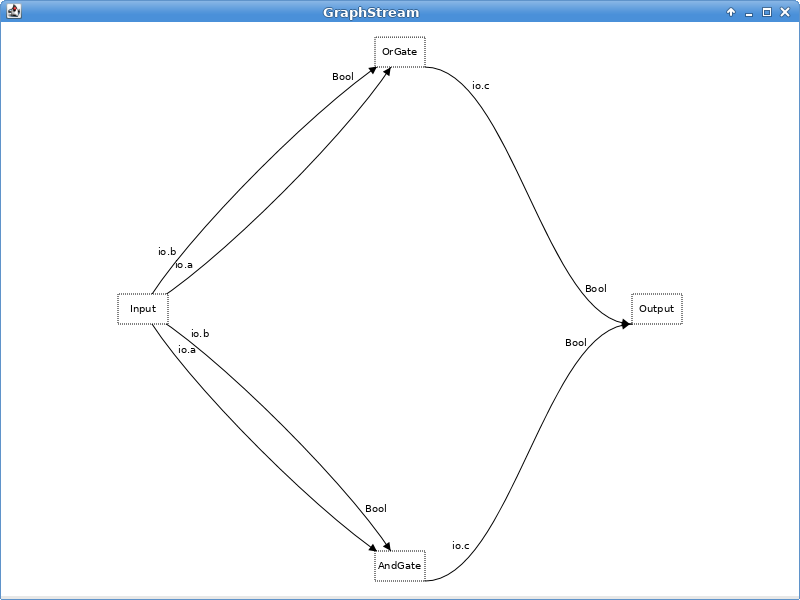
\includegraphics[width=0.8\textwidth]{img/graphstream-base-model-example}
  \caption{The base graph model rendering using graphstream}
  \label{fig:base-graph-model-graphstream}
\end{figure}

GraphStream allow us to simply create a graph (or a multigraph) in Java like in listing \ref{lst:graphstream-example}.

\begin{listing}[p]
  \centering
  \begin{javacode}
    public class Example
    {
      public static void main(String args[])
      {
        Graph graph = new SingleGraph("Example");
        graph.addNode("A" );
        graph.addNode("B" );
        graph.addNode("C" );
        graph.addEdge("AB", "A", "B");
        graph.addEdge("BC", "B", "C");
        graph.addEdge("CA", "C", "A");
      }
    }
  \end{javacode}
  \caption[A simple graph modelisation using GraphStream]{Modelisation of a simple graph using the GraphStream library}
  \label{lst:graphstream-example}
\end{listing}


\subsection{Remarks}
\label{sub:Remarks}

With GraphStream, there is no way to control some visual features which are very interresing for hardware component visualisation :
the splines of the edges and the anchor position on the node.
There is no way to have a node with sub-node like in the base graph model in figure \ref{fig:graph-base-model}.

An another special case is the label on the edges.
With GraphStream, we could add some label on the edges like in listings \ref{lst:graphstream-edge-label}, but we can't add multiple ones.
To add multiple label we need to use sprite like in listing \ref{lst:graphstream-edge-sprite}.

\begin{listing}[p]
  \centering
  \javafile{../ViewingLibrary/GraphstreamTest/src/examples/EdgesLabel.java}
  \caption[Add a label on an edge with GraphStream]{TODO : maybe remove ?}
  \label{lst:graphstream-edge-label}
\end{listing}

\begin{listing}[p]
  \centering
  \javafile{../ViewingLibrary/GraphstreamTest/src/examples/SpriteEdgesExample.java}
  \caption[Add two label on an edge with GraphStream]{TODO : maybe remove ?}
  \label{lst:graphstream-edge-sprite}
\end{listing}


\subsection{Conclusion}
\label{sub:Conclusion-gs}

GraphStream ownes some another features which could be usefull to design an application :
\begin{itemize}
\item View integration using Swing
\item Human-Computer interaction with the view
\item A complete CSS interpretation to personalize the nodes and the edges
\end{itemize}

The main problem using GraphStream is we need to indicates the component information using label on the edges. The figure \ref{fig:base-graph-model-graphstream} show four nodes and six connections, but
if we have a more lot of edges between nodes, it would be difficult to see the type of the inputs and outputs, like show in figure \ref{fig:graphstream-lot-of-edges}.

\begin{figure}[h]
  \centering
  \fbox{
    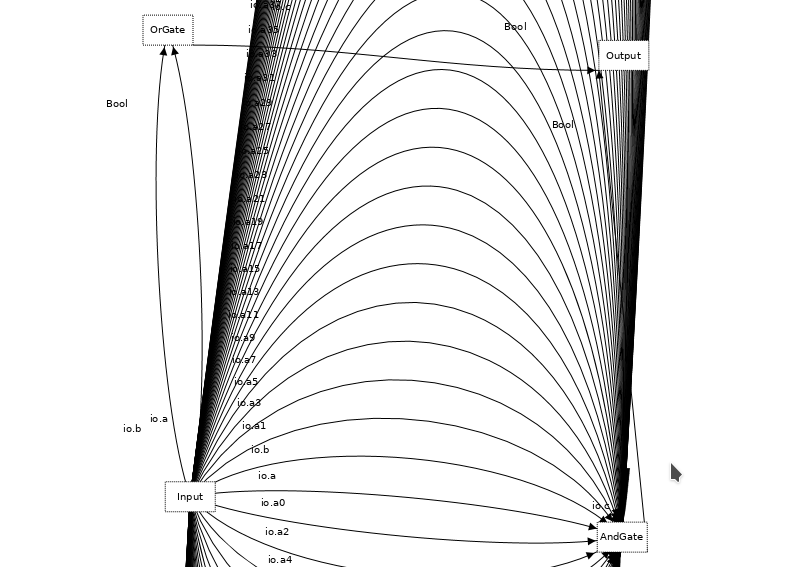
\includegraphics[width=0.8\textwidth]{img/graphstream_lot_of_edges}
  }
  \caption[Label on multiple edges using GraphStream]{}
  \label{fig:graphstream-lot-of-edges}
\end{figure}

In order to overpass these problem, we need to visualize the type in an another form : in the graph \ref{fig:graph-base-model} we have the idea to show the inputs and outputs as a port of the component. With GraphStream we can't do that, so we need to an another library which have these idea of port.



\section{Draw2D}
\label{sec:Draw2D}

Draw2D is a HTML5 and Javascript library for visualization and interaction with diagrams and graph\cite{draw2d}. The goal of the library is to provide a way to represent diagrams and graph and manipulate those using the mouse or javascript code. Some existing product already use Draw2d for diagrams manipulation :

\begin{itemize}
\item Shape Designer\cite{draw2d}
\item BrainBox\cite{draw2d}
\item Sankey State\cite{draw2d}
\end{itemize}

\subsection{Implementation of the base graph model}
\label{sub:Implementation of the base graph model}

Before implementing directly the basic example of the graph \ref{fig:graph-base-model},
we need to extend the library with a new component for our usage.
In the chapter \ref{sub:Conclusion-gs} we indicates that's the GraphStream library is lacking the idea of port, but Draw2d already have those.

The listing \ref{lst:draw2d-base-graph-model} show the realisation of the base graph model example.
Note that the object \textbf{ComponentShape} and the functions \textbf{ComponentShape.addPort()},\textbf{newConnection()} and
\textbf{createConnection()} are not part of the Draw2d library, it's an extension added for this project. Those implementation are discuss in the section \ref{sec:Extension of the Draw2d library}.

\begin{listing}[p]
  \centering
  \begin{jscode}
    var canvas = new draw2d.Canvas("gfx_holder1");

    var andGate = new ComponentShape();
    var orGate = new ComponentShape();
    var input = new ComponentShape();
    var output = new ComponentShape();

    canvas.installEditPolicy(new draw2d.policy.connection.DragConnectionCreatePolicy({
      createConnection: createConnection
    }));

    andGate.setName("AndGate");
    orGate.setName("OrGate");
    input.setName("Input");
    output.setName("Output");

    andGate.addPort("io.a", "input");
    andGate.addPort("io.b", "input");
    andGate.addPort("io.c", "output");

    orGate.addPort("io.a", "input");
    orGate.addPort("io.b", "input");
    orGate.addPort("io.c", "output");

    input.addPort("io.a", "output");
    input.addPort("io.b", "output");

    output.addPort("io.c", "input");

    canvas.add(input);
    canvas.add(output);
    canvas.add(andGate);
    canvas.add(orGate);

    canvas.add(newConnection(input.getPort("io.a"), andGate.getPort("io.a")));
    canvas.add(newConnection(input.getPort("io.b"), andGate.getPort("io.b")));
    canvas.add(newConnection(input.getPort("io.a"), orGate.getPort("io.a")));
    canvas.add(newConnection(input.getPort("io.b"), orGate.getPort("io.b")));
    canvas.add(newConnection(andGate.getPort("io.c"), output.getPort("io.c")));
    canvas.add(newConnection(orGate.getPort("io.c"), output.getPort("io.c")));
  \end{jscode}

  \caption[Base graph model implementation using the Draw2D library]{The necessary code to produce the base graph model with the Draw2d library.
    The object \textbf{ComponentShape} and the functions \textbf{addPort()},  \textbf{newConnection()} and \textbf{createConnection()} are not part of the Draw2d library, it's an extension added for this project.}

  \label{lst:draw2d-base-graph-model}
\end{listing}

The code \ref{lst:draw2d-base-graph-model} is producing the HTML page see in figure \ref{fig:base-graph-model-html-draw2d}.

\begin{figure}[h]
  \centering
  \fbox{
    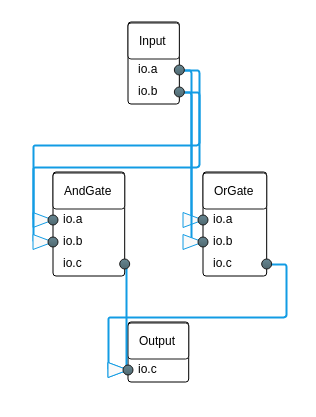
\includegraphics[width=0.5\textwidth]{img/draw2d-base-model-example}
  }
  \caption[Render of the base graph model using the Draw2D library]{Rendering of the base graph model diagram from figure \ref{fig:graph-base-model} using the Draw2D library}
  \label{fig:base-graph-model-html-draw2d}
\end{figure}



\section{Graph layout}
\label{sec:graph-layout}

One functionnality the Draw2D don't have is the layout of the diagram. If we said nothing about the position of the node, Draw2D simply overlap all the nodes and manage nothing for the visualization like in figure \ref{fig:draw2d_overlapping}.

\begin{figure}
  \centering
  \fbox{
    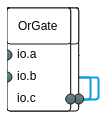
\includegraphics{img/overlap_draw2d}
  }
  \caption[Overlapping of nodes by Draw2D]{When we specify nothing about the node position with Draw2D, the engine just overlaps all the node}
  \label{fig:draw2d_overlapping}
\end{figure}

In order to produce a visualisable diagram, we need to layout ourself the diagram. We need to mention that's the layout algorithm is a NP-Hard problem in computing theory\cite{Tamassia:2007:HGD:1202383} and for our graph, we have some specialties :

\begin{itemize}
\item The graph could be cyclic
\item The graph is oriented
\item Nodes ownes port, so we need to layout the edges on specific part of the graph
\end{itemize}

The first two specialties aren't a big deal, but the last one is quiet problematic, he involved a special layout algorithm which take care of the ports position on the nodes. Otherwise the visual result could be chaotics like in figure \ref{fig:multigraph-no-port}, in which we can't see the connection between some specific ports.

\begin{figure}[h]
  \centering
  \fbox{
    \digraph[scale=0.5]{MultiGraphNoPort}{
      A -> B -> C -> D;
      A -> B -> C;
      A -> B;
      D -> A;
      D -> B;
    }
  }
  \caption[Visualization of a multi-graph without port]{Visualization of a multi-graph without port, we could not determine the connection which is representing a certain connection between two component}
  \label{fig:multigraph-no-port}
\end{figure}

In order to solve this drawback, we need to layout the graph ourself by using a
library. We could also do it ourself by implementing the algorithm for the kind
of graph we have, but it's to time-consuming for a project like this.

TODO layout des edges du graph... (questions sur le forum de Draw2d.org)

